% Preamble
\documentclass[10pt,letterpaper]{article}
\usepackage[spanish]{babel}

% Packages
\selectlanguage{spanish}
\usepackage[utf8]{inputenc} % For spanish (and international) letters like acents.
\usepackage{hyperref} % To create hyperlinks within the document.
\hypersetup{ % Custome options for package hyperref:
	colorlinks=true, % Links without borders
	linkcolor=black, % Internal links (black index)
	urlcolor=blue % External links
}
\usepackage{graphicx} % To include graphics (pictures, images)
\usepackage{float} % For the use of the parameter "H" in command "\begin{figure}[H]" (i.e. exact position of image in text)
\usepackage{tabularx} % Similar to tabular* environment, for width and stretching in tables
\usepackage[table]{xcolor} % Color in cell [http://ctan.org/pkg/xcolor]
\definecolor{NewBlue}{RGB}{102, 153, 255}
\usepackage[strict]{changepage} % Allow to change margins (like \textwidth). 
% By the way, about page size and margins: https://www.sharelatex.com/learn/Page_size_and_margins

% Document environment
\begin{document}

% Top matter
\title{Documentación de los Requerimientos del Sistema de apoyo a la catalogación de archivos audiovisuales del LAIS}
\author{Rodrigo Eduardo Colín Rivera, Sergio Amaro Rosas}
\date{\today}
\maketitle

\begin{abstract}
La siguiente documentación tiene como objetivo \ldots
\end{abstract}

\tableofcontents % Indice
\newpage

\setcounter{secnumdepth}{0} % Non-numbering sections
\setcounter{tocdepth}{0} % Non-numnbering table of contents
\graphicspath{{../Diagramas/}{../Screenshots}} % Path of the folders containing the images

\section{Enunciado del problema}

\section{Diagrama general de casos de uso}
\begin{figure}[H]
	\centering
	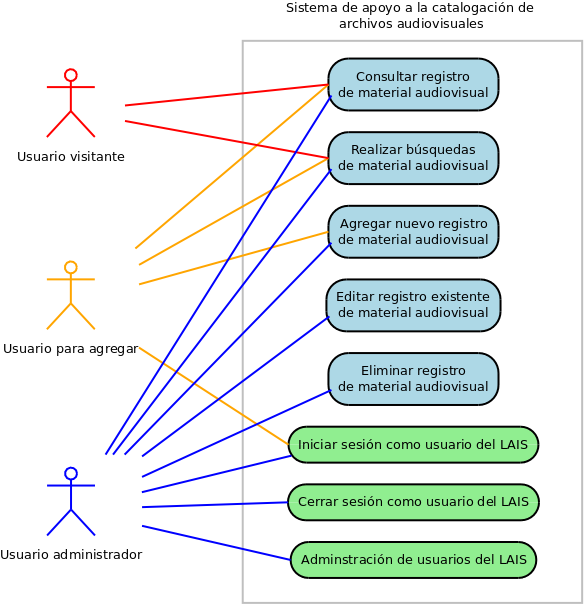
\includegraphics[width=0.8\textwidth]{CasosDeUso.png}
	\caption{Diagrama de casos de uso}
	\label{fig:caso_de_uso}
\end{figure}

\section{Casos de uso detallados, casos de prueba, prototipo de interfaz}

\subsection{Usuario visitante}

\subsubsection{Consultar información de archivo audiovisual}
% Actor
\textbf{Actor:} Usuario visitante

% Imagen del diagrama específico del caso
\begin{figure}[H]
	\centering
	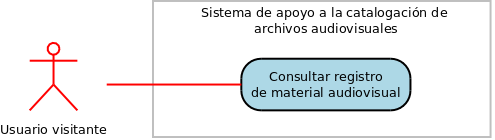
\includegraphics[width=0.8\textwidth]{CasoDeUso_Visitante_ConsultarRegistro.png}
\end{figure}

% Descripción
\textbf{Descipción: } Acción que permite mostrar la información completa de un archivo audiovisual cuya portada es mostrada en pantalla.

% Precondiciones
\textbf{Precondiciones:} Estar en alguna de las páginas que muestra los archivos audiovisuales por década.

% Flujo Normal de Eventos (tabla)
\begin{adjustwidth}{-6em}{-6em}
	\begin{center}
		\begin{tabularx}{1.2\textwidth}{ | p{0.7cm} | X | p{0.7cm} | X | p{1.5cm} | }
			\hline
			\rowcolor{NewBlue} \multicolumn{5}{|c|}{\textbf{Flujo normal de eventos}} \\
			\hline
			\multicolumn{2}{|c|}{\textbf{Actor(es)}}	&	\multicolumn{2}{c|}{\textbf{Sistema}}	&	\textbf{Alterno} \\
			\hline
			\textbf{Paso}	&	\textbf{Acción}	&	\textbf{Paso}	&	\textbf{Acción}	&	\textbf{ID} \\
			\hline
			1 & 
			Dar clic en la portada del audiovisual que se desea ver &
			2 &
			El sistema pide todos los datos del audiovisual a la base de datos &
			E1 \\
			\hline
			& 
			&
			3 &
			El sistema muestra una ventana emergente con toda la información del audiovisual. & 
			A1 \\
			\hline
		\end{tabularx}
	\end{center}
\end{adjustwidth}

% Flujo Alterno (en caso de ser necesario)
\begin{adjustwidth}{-6em}{-6em}
	\begin{center}
		\begin{tabularx}{1.2\textwidth}{ | p{0.6cm} | X | X | }
			\hline
			\rowcolor{NewBlue} \multicolumn{3}{|c|}{\textbf{Flujo alterno de eventos}} \\
			\hline
			\textbf{ID}	&	\textbf{Descripción}	&	\textbf{Acción} \\
			\hline
			A1 &
			El usuario da clic en el botón de ``Ver más'' para ver información específica del archivo audiovisual &
			El sistema muestra en la parte inferior toda la información disponible del archivo audiovisual separada por áreas. \\
			\hline
		\end{tabularx}
	\end{center}
\end{adjustwidth}

% Flujo de Excepcion de Eventos (tabla)
\begin{adjustwidth}{-6em}{-6em}
	\begin{center}
		\begin{tabularx}{1.2\textwidth}{ | p{0.6cm} | X | X | }
			\hline
			\rowcolor{NewBlue} \multicolumn{3}{|c|}{\textbf{Flujo excepcional de eventos}} \\
			\hline
			\textbf{ID}	&	\textbf{Descripción}	&	\textbf{Acción} \\
			\hline
			E1 &
			No hay conexión con la base de datos. &
			El sistema devuelve un mensaje de error de conexión. \\
			\hline
		\end{tabularx}
	\end{center}
\end{adjustwidth}

% Post-condiciones
\textbf{Postcondiciones:} El entorno de la página se oscurece para dar enfoque a la información completa del archivo audiovisual.

% Casos de prueba para flujo normal (tabla) y su prototipo (imagen)
%\begin{figure}[H]
%	\centering
%	\includegraphics[width=0.8\textwidth]{imagen.png}
%\end{figure}

\begin{adjustwidth}{-6em}{-6em}
	\begin{center}
		\begin{tabularx}{1.2\textwidth}{ | X | X | }
			\hline
			\rowcolor{NewBlue} \multicolumn{2}{|c|}{\textbf{Casos de prueba (Flujo normal)}} \\
			\hline
			\textbf{Entradas}	&	\textbf{Resultado esperado} \\
			\hline
			Clic en una portada de audiovisual. &
			Mostrar el contenido completo del archivo audiovisual seleccionado. \\
			\hline
		\end{tabularx}
	\end{center}
\end{adjustwidth}

% Casos de prueba (Flujo alterno de eventos) [cuando es necesario]

%\begin{figure}[H]
%	\centering
%	\includegraphics[width=0.8\textwidth]{imagen.png}
%\end{figure}

\begin{adjustwidth}{-6em}{-6em}
	\begin{center}
		\begin{tabularx}{1.2\textwidth}{ | p{0.6cm} | X | X | }
			\hline
			\rowcolor{NewBlue} \multicolumn{3}{|c|}{\textbf{Caso de prueba (Flujo alterno)}} \\
			\hline
			\textbf{ID}	&	\textbf{Entrada}	&	\textbf{Resultado esperado} \\
			\hline
			A1 &
			Clic en el botón de ``Ver más''. &
			El sistema muestra en la parte inferior toda la información disponible del archivo audiovisual separada por áreas. \\
			\hline
		\end{tabularx}
	\end{center}
\end{adjustwidth}

% Casos de prueba para excepción de eventos (tabla) y su prototipo (imagen)
%\begin{figure}[H]
%	\centering
%	\includegraphics[width=0.8\textwidth]{imagen.png}
%\end{figure}

\begin{adjustwidth}{-6em}{-6em}
	\begin{center}
		\begin{tabularx}{1.2\textwidth}{ | p{0.6cm} | X | X | }
			\hline
			\rowcolor{NewBlue} \multicolumn{3}{|c|}{\textbf{Caso de prueba (Flujo excepcional)}} \\
			\hline
			\textbf{ID}	&	\textbf{Entrada}	&	\textbf{Resultado esperado} \\
			\hline
			E1 &
			Clic en una portada de audiovisual. &
			El sistema devuelve un mensaje de error de conexión. \\
			\hline
		\end{tabularx}
	\end{center}
\end{adjustwidth}

\subsubsection{Realizar búsqueda de material audiovisual}
% Actor
\textbf{Actor:} Usuario visitante

% Imagen del diagrama específico del caso
\begin{figure}[H]
	\centering
	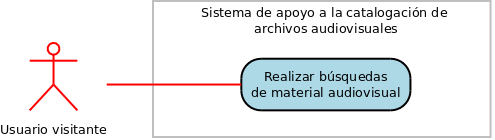
\includegraphics[width=0.8\textwidth]{CasoDeUso_Visitante_Busqueda.png}
\end{figure}

% Descripción
\textbf{Descipción: } Acción que permite realizar una búsqueda de material audiovisual.

% Precondiciones
\textbf{Precondiciones:} Estar en cualquiera de las páginas del sistema.

% Flujo Normal de Eventos (tabla)
\begin{adjustwidth}{-6em}{-6em}
	\begin{center}
		\begin{tabularx}{1.2\textwidth}{ | p{0.7cm} | X | p{0.7cm} | X | p{1.5cm} | }
			\hline
			\rowcolor{NewBlue} \multicolumn{5}{|c|}{\textbf{Flujo normal de eventos}} \\
			\hline
			\multicolumn{2}{|c|}{\textbf{Actor(es)}}	&	\multicolumn{2}{c|}{\textbf{Sistema}}	&	\textbf{Alterno} \\
			\hline
			\textbf{Paso}	&	\textbf{Acción}	&	\textbf{Paso}	&	\textbf{Acción}	&	\textbf{ID} \\
			\hline
			1 & 
			Escribir texto de búsqueda en el campo situado en la parte superior del navegador y presionar \textit{Enter} en el teclado o clic en el botón con el icono de lupa situado a la derecha &
			2 &
			El sistema realiza una búsqueda dentro de la base de datos con las coincidencias de las palabras escritas &
			E1 \\
			\hline
			& 
			&
			3 &
			El sistema muestra los resultados en pantalla utilizando la misma vista que los archivos audiovisuales por década (mostrando la portada, el título y el año) & 
			E2\\
			\hline
		\end{tabularx}
	\end{center}
\end{adjustwidth}

% Flujo de Excepcion de Eventos (tabla)
\begin{adjustwidth}{-6em}{-6em}
	\begin{center}
		\begin{tabularx}{1.2\textwidth}{ | p{0.6cm} | X | X | }
			\hline
			\rowcolor{NewBlue} \multicolumn{3}{|c|}{\textbf{Flujo excepcional de eventos}} \\
			\hline
			\textbf{ID}	&	\textbf{Descripción}	&	\textbf{Acción} \\
			\hline
			E1 &
			No hay conexión con la base de datos. &
			El sistema devuelve un mensaje de error de conexión. \\
			\hline
			E2 &
			No hay coincidencias de búsqueda en la base de datos. &
			El sistema muestra un texto indicando no hay resultados de la búsqueda. \\
			\hline
		\end{tabularx}
	\end{center}
\end{adjustwidth}

% Post-condiciones
\textbf{Postcondiciones:} El usuario es autodirigido a la página que muestra los audiovisuales resultantes de la búsqueda.

% Casos de prueba para flujo normal (tabla) y su prototipo (imagen)
%\begin{figure}[H]
%	\centering
%	\includegraphics[width=0.8\textwidth]{imagen.png}
%\end{figure}

\begin{adjustwidth}{-6em}{-6em}
	\begin{center}
		\begin{tabularx}{1.2\textwidth}{ | X | X | }
			\hline
			\rowcolor{NewBlue} \multicolumn{2}{|c|}{\textbf{Casos de prueba (Flujo normal)}} \\
			\hline
			\textbf{Entradas}	&	\textbf{Resultado esperado} \\
			\hline
			Escribir texto de búsqueda y presionar \textit{Enter} en el teclado o dar clic en el botón de búsqueda &
			El sistema muestra los audiovisuales resultantes en pantalla. \\
			\hline
		\end{tabularx}
	\end{center}
\end{adjustwidth}

% Casos de prueba para excepción de eventos (tabla) y su prototipo (imagen)
%\begin{figure}[H]
%	\centering
%	\includegraphics[width=0.8\textwidth]{imagen.png}
%\end{figure}

\begin{adjustwidth}{-6em}{-6em}
	\begin{center}
		\begin{tabularx}{1.2\textwidth}{ | p{0.6cm} | X | X | }
			\hline
			\rowcolor{NewBlue} \multicolumn{3}{|c|}{\textbf{Caso de prueba (Flujo excepcional)}} \\
			\hline
			\textbf{ID}	&	\textbf{Entrada}	&	\textbf{Resultado esperado} \\
			\hline
			E1 &
			No hay conexión con la base de datos. &
			El sistema devuelve un mensaje de error de conexión. \\
			\hline
			E2 &
			No hay coincidencias de búsqueda en la base de datos. &
			El sistema muestra un texto indicando no hay resultados de la búsqueda. \\
			\hline
		\end{tabularx}
	\end{center}
\end{adjustwidth}

\subsection{Usuario con permisos para agregar}

\subsubsection{Consultar registro de material audiovisual}
% Actor
\textbf{Actor:} Usuario para agregar

% Imagen del diagrama específico del caso
\begin{figure}[H]
	\centering
	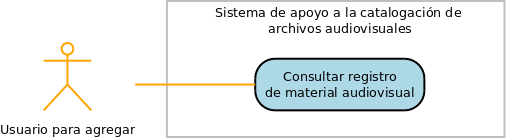
\includegraphics[width=0.8\textwidth]{CasoDeUso_Agregar_ConsultarRegistro.png}
\end{figure}

% Descripción
\textbf{Descipción: } Acción que permite mostrar la información completa de un archivo audiovisual cuya portada es mostrada en pantalla.

% Precondiciones
\textbf{Precondiciones:} Estar en alguna de las páginas que muestra los archivos audiovisuales por década.

% Flujo Normal de Eventos (tabla)
\begin{adjustwidth}{-6em}{-6em}
	\begin{center}
		\begin{tabularx}{1.2\textwidth}{ | p{0.7cm} | X | p{0.7cm} | X | p{1.5cm} | }
			\hline
			\rowcolor{NewBlue} \multicolumn{5}{|c|}{\textbf{Flujo normal de eventos}} \\
			\hline
			\multicolumn{2}{|c|}{\textbf{Actor(es)}}	&	\multicolumn{2}{c|}{\textbf{Sistema}}	&	\textbf{Alterno} \\
			\hline
			\textbf{Paso}	&	\textbf{Acción}	&	\textbf{Paso}	&	\textbf{Acción}	&	\textbf{ID} \\
			\hline
			1 & 
			Dar clic en la portada del audiovisual que se desea ver &
			2 &
			El sistema pide todos los datos del audiovisual a la base de datos &
			E1 \\
			\hline
			& 
			&
			3 &
			El sistema muestra una ventana emergente con toda la información del audiovisual. & 
			A1 \\
			\hline
		\end{tabularx}
	\end{center}
\end{adjustwidth}

% Flujo Alterno (en caso de ser necesario)
\begin{adjustwidth}{-6em}{-6em}
	\begin{center}
		\begin{tabularx}{1.2\textwidth}{ | p{0.6cm} | X | X | }
			\hline
			\rowcolor{NewBlue} \multicolumn{3}{|c|}{\textbf{Flujo alterno de eventos}} \\
			\hline
			\textbf{ID}	&	\textbf{Descripción}	&	\textbf{Acción} \\
			\hline
			A1 &
			El usuario da clic en el botón de ``Ver más'' para ver información específica del archivo audiovisual &
			El sistema muestra en la parte inferior toda la información disponible del archivo audiovisual separada por áreas. \\
			\hline
		\end{tabularx}
	\end{center}
\end{adjustwidth}

% Flujo de Excepcion de Eventos (tabla)
\begin{adjustwidth}{-6em}{-6em}
	\begin{center}
		\begin{tabularx}{1.2\textwidth}{ | p{0.6cm} | X | X | }
			\hline
			\rowcolor{NewBlue} \multicolumn{3}{|c|}{\textbf{Flujo excepcional de eventos}} \\
			\hline
			\textbf{ID}	&	\textbf{Descripción}	&	\textbf{Acción} \\
			\hline
			E1 &
			No hay conexión con la base de datos. &
			El sistema devuelve un mensaje de error de conexión. \\
			\hline
		\end{tabularx}
	\end{center}
\end{adjustwidth}

% Post-condiciones
\textbf{Postcondiciones:} El entorno de la página se oscurece para dar enfoque a la información completa del archivo audiovisual.

% Casos de prueba para flujo normal (tabla) y su prototipo (imagen)
%\begin{figure}[H]
%	\centering
%	\includegraphics[width=0.8\textwidth]{imagen.png}
%\end{figure}

\begin{adjustwidth}{-6em}{-6em}
	\begin{center}
		\begin{tabularx}{1.2\textwidth}{ | X | X | }
			\hline
			\rowcolor{NewBlue} \multicolumn{2}{|c|}{\textbf{Casos de prueba (Flujo normal)}} \\
			\hline
			\textbf{Entradas}	&	\textbf{Resultado esperado} \\
			\hline
			Clic en una portada de audiovisual. &
			Mostrar el contenido completo del archivo audiovisual seleccionado. \\
			\hline
		\end{tabularx}
	\end{center}
\end{adjustwidth}

% Casos de prueba (Flujo alterno de eventos) [cuando es necesario]

%\begin{figure}[H]
%	\centering
%	\includegraphics[width=0.8\textwidth]{imagen.png}
%\end{figure}

\begin{adjustwidth}{-6em}{-6em}
	\begin{center}
		\begin{tabularx}{1.2\textwidth}{ | p{0.6cm} | X | X | }
			\hline
			\rowcolor{NewBlue} \multicolumn{3}{|c|}{\textbf{Caso de prueba (Flujo alterno)}} \\
			\hline
			\textbf{ID}	&	\textbf{Entrada}	&	\textbf{Resultado esperado} \\
			\hline
			A1 &
			Clic en el botón de ``Ver más''. &
			El sistema muestra en la parte inferior toda la información disponible del archivo audiovisual separada por áreas. \\
			\hline
		\end{tabularx}
	\end{center}
\end{adjustwidth}

% Casos de prueba para excepción de eventos (tabla) y su prototipo (imagen)
%\begin{figure}[H]
%	\centering
%	\includegraphics[width=0.8\textwidth]{imagen.png}
%\end{figure}

\begin{adjustwidth}{-6em}{-6em}
	\begin{center}
		\begin{tabularx}{1.2\textwidth}{ | p{0.6cm} | X | X | }
			\hline
			\rowcolor{NewBlue} \multicolumn{3}{|c|}{\textbf{Caso de prueba (Flujo excepcional)}} \\
			\hline
			\textbf{ID}	&	\textbf{Entrada}	&	\textbf{Resultado esperado} \\
			\hline
			E1 &
			Clic en una portada de audiovisual. &
			El sistema devuelve un mensaje de error de conexión. \\
			\hline
		\end{tabularx}
	\end{center}
\end{adjustwidth}

\subsubsection{Realizar búsquedas de material audiovisual}
% Actor
\textbf{Actor:} Usuario para agregar

% Imágen del diagrama específico del caso
\begin{figure}[H]
	\centering
	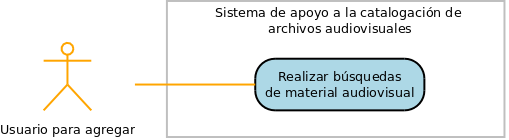
\includegraphics[width=0.8\textwidth]{CasoDeUso_Agregar_Busqueda.png}
\end{figure}

% Descripción
\textbf{Descipción: } Acción que permite realizar una búsqueda de material audiovisual.

% Precondiciones
\textbf{Precondiciones:} Estar en cualquiera de las páginas del sistema.

% Flujo Normal de Eventos (tabla)
\begin{adjustwidth}{-6em}{-6em}
	\begin{center}
		\begin{tabularx}{1.2\textwidth}{ | p{0.7cm} | X | p{0.7cm} | X | p{1.5cm} | }
			\hline
			\rowcolor{NewBlue} \multicolumn{5}{|c|}{\textbf{Flujo normal de eventos}} \\
			\hline
			\multicolumn{2}{|c|}{\textbf{Actor(es)}}	&	\multicolumn{2}{c|}{\textbf{Sistema}}	&	\textbf{Alterno} \\
			\hline
			\textbf{Paso}	&	\textbf{Acción}	&	\textbf{Paso}	&	\textbf{Acción}	&	\textbf{ID} \\
			\hline
			1 & 
			Escribir texto de búsqueda en el campo situado en la parte superior del navegador y presionar \textit{Enter} en el teclado o clic en el botón con el icono de lupa situado a la derecha &
			2 &
			El sistema realiza una búsqueda dentro de la base de datos con las coincidencias de las palabras escritas &
			E1 \\
			\hline
			& 
			&
			3 &
			El sistema muestra los resultados en pantalla utilizando la misma vista que los archivos audiovisuales por década (mostrando la portada, el título y el año) & 
			E2\\
			\hline
		\end{tabularx}
	\end{center}
\end{adjustwidth}

% Flujo de Excepcion de Eventos (tabla)
\begin{adjustwidth}{-6em}{-6em}
	\begin{center}
		\begin{tabularx}{1.2\textwidth}{ | p{0.6cm} | X | X | }
			\hline
			\rowcolor{NewBlue} \multicolumn{3}{|c|}{\textbf{Flujo excepcional de eventos}} \\
			\hline
			\textbf{ID}	&	\textbf{Descripción}	&	\textbf{Acción} \\
			\hline
			E1 &
			No hay conexión con la base de datos. &
			El sistema devuelve un mensaje de error de conexión. \\
			\hline
			E2 &
			No hay coincidencias de búsqueda en la base de datos. &
			El sistema muestra un texto indicando no hay resultados de la búsqueda. \\
			\hline
		\end{tabularx}
	\end{center}
\end{adjustwidth}

% Post-condiciones
\textbf{Postcondiciones:} El usuario es autodirigido a la página que muestra los audiovisuales resultantes de la búsqueda.

% Casos de prueba para flujo normal (tabla) y su prototipo (imagen)
%\begin{figure}[H]
%	\centering
%	\includegraphics[width=0.8\textwidth]{imagen.png}
%\end{figure}

\begin{adjustwidth}{-6em}{-6em}
	\begin{center}
		\begin{tabularx}{1.2\textwidth}{ | X | X | }
			\hline
			\rowcolor{NewBlue} \multicolumn{2}{|c|}{\textbf{Casos de prueba (Flujo normal)}} \\
			\hline
			\textbf{Entradas}	&	\textbf{Resultado esperado} \\
			\hline
			Escribir texto de búsqueda y presionar \textit{Enter} en el teclado o dar clic en el botón de búsqueda &
			El sistema muestra los audiovisuales resultantes en pantalla. \\
			\hline
		\end{tabularx}
	\end{center}
\end{adjustwidth}

% Casos de prueba para excepción de eventos (tabla) y su prototipo (imagen)
%\begin{figure}[H]
%	\centering
%	\includegraphics[width=0.8\textwidth]{imagen.png}
%\end{figure}

\begin{adjustwidth}{-6em}{-6em}
	\begin{center}
		\begin{tabularx}{1.2\textwidth}{ | p{0.6cm} | X | X | }
			\hline
			\rowcolor{NewBlue} \multicolumn{3}{|c|}{\textbf{Caso de prueba (Flujo excepcional)}} \\
			\hline
			\textbf{ID}	&	\textbf{Entrada}	&	\textbf{Resultado esperado} \\
			\hline
			E1 &
			No hay conexión con la base de datos. &
			El sistema devuelve un mensaje de error de conexión. \\
			\hline
			E2 &
			No hay coincidencias de búsqueda en la base de datos. &
			El sistema muestra un texto indicando no hay resultados de la búsqueda. \\
			\hline
		\end{tabularx}
	\end{center}
\end{adjustwidth}

\subsubsection{Agregar nuevo registro de material audiovisual}
% Actor
\textbf{Actor:} Usuario para agregar

\subsubsection{Iniciar sesion como usuario de LAIS}
% Actor
\textbf{Actor:} Usuario para agregar

\subsubsection{Cerrar sesion como usuario del LAIS}
% Actor
\textbf{Actor:} Usuario para agregar

\subsection{Usuario administrador}

\subsubsection{Consultar registro de material audiovisual}
% Actor
\textbf{Actor:} Usuario administrador

% Imagen del diagrama específico del caso
\begin{figure}[H]
	\centering
	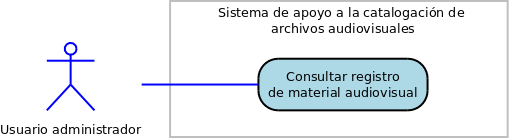
\includegraphics[width=0.8\textwidth]{CasoDeUso_Administrador_ConsultarRegistro.png}
\end{figure}

% Descripción
\textbf{Descipción: } Acción que permite mostrar la información completa de un archivo audiovisual cuya portada es mostrada en pantalla.

% Precondiciones
\textbf{Precondiciones:} Estar en alguna de las páginas que muestra los archivos audiovisuales por década.

% Flujo Normal de Eventos (tabla)
\begin{adjustwidth}{-6em}{-6em}
	\begin{center}
		\begin{tabularx}{1.2\textwidth}{ | p{0.7cm} | X | p{0.7cm} | X | p{1.5cm} | }
			\hline
			\rowcolor{NewBlue} \multicolumn{5}{|c|}{\textbf{Flujo normal de eventos}} \\
			\hline
			\multicolumn{2}{|c|}{\textbf{Actor(es)}}	&	\multicolumn{2}{c|}{\textbf{Sistema}}	&	\textbf{Alterno} \\
			\hline
			\textbf{Paso}	&	\textbf{Acción}	&	\textbf{Paso}	&	\textbf{Acción}	&	\textbf{ID} \\
			\hline
			1 & 
			Dar clic en la portada del audiovisual que se desea ver &
			2 &
			El sistema pide todos los datos del audiovisual a la base de datos &
			E1 \\
			\hline
			& 
			&
			3 &
			El sistema muestra una ventana emergente con toda la información del audiovisual. & 
			A1 \\
			\hline
		\end{tabularx}
	\end{center}
\end{adjustwidth}

% Flujo Alterno (en caso de ser necesario)
\begin{adjustwidth}{-6em}{-6em}
	\begin{center}
		\begin{tabularx}{1.2\textwidth}{ | p{0.6cm} | X | X | }
			\hline
			\rowcolor{NewBlue} \multicolumn{3}{|c|}{\textbf{Flujo alterno de eventos}} \\
			\hline
			\textbf{ID}	&	\textbf{Descripción}	&	\textbf{Acción} \\
			\hline
			A1 &
			El usuario da clic en el botón de ``Ver más'' para ver información específica del archivo audiovisual &
			El sistema muestra en la parte inferior toda la información disponible del archivo audiovisual separada por áreas. \\
			\hline
		\end{tabularx}
	\end{center}
\end{adjustwidth}

% Flujo de Excepcion de Eventos (tabla)
\begin{adjustwidth}{-6em}{-6em}
	\begin{center}
		\begin{tabularx}{1.2\textwidth}{ | p{0.6cm} | X | X | }
			\hline
			\rowcolor{NewBlue} \multicolumn{3}{|c|}{\textbf{Flujo excepcional de eventos}} \\
			\hline
			\textbf{ID}	&	\textbf{Descripción}	&	\textbf{Acción} \\
			\hline
			E1 &
			No hay conexión con la base de datos. &
			El sistema devuelve un mensaje de error de conexión. \\
			\hline
		\end{tabularx}
	\end{center}
\end{adjustwidth}

% Post-condiciones
\textbf{Postcondiciones:} El entorno de la página se oscurece para dar enfoque a la información completa del archivo audiovisual.

% Casos de prueba para flujo normal (tabla) y su prototipo (imagen)
%\begin{figure}[H]
%	\centering
%	\includegraphics[width=0.8\textwidth]{imagen.png}
%\end{figure}

\begin{adjustwidth}{-6em}{-6em}
	\begin{center}
		\begin{tabularx}{1.2\textwidth}{ | X | X | }
			\hline
			\rowcolor{NewBlue} \multicolumn{2}{|c|}{\textbf{Casos de prueba (Flujo normal)}} \\
			\hline
			\textbf{Entradas}	&	\textbf{Resultado esperado} \\
			\hline
			Clic en una portada de audiovisual. &
			Mostrar el contenido completo del archivo audiovisual seleccionado. \\
			\hline
		\end{tabularx}
	\end{center}
\end{adjustwidth}

% Casos de prueba (Flujo alterno de eventos) [cuando es necesario]

%\begin{figure}[H]
%	\centering
%	\includegraphics[width=0.8\textwidth]{imagen.png}
%\end{figure}

\begin{adjustwidth}{-6em}{-6em}
	\begin{center}
		\begin{tabularx}{1.2\textwidth}{ | p{0.6cm} | X | X | }
			\hline
			\rowcolor{NewBlue} \multicolumn{3}{|c|}{\textbf{Caso de prueba (Flujo alterno)}} \\
			\hline
			\textbf{ID}	&	\textbf{Entrada}	&	\textbf{Resultado esperado} \\
			\hline
			A1 &
			Clic en el botón de ``Ver más''. &
			El sistema muestra en la parte inferior toda la información disponible del archivo audiovisual separada por áreas. \\
			\hline
		\end{tabularx}
	\end{center}
\end{adjustwidth}

% Casos de prueba para excepción de eventos (tabla) y su prototipo (imagen)
%\begin{figure}[H]
%	\centering
%	\includegraphics[width=0.8\textwidth]{imagen.png}
%\end{figure}

\begin{adjustwidth}{-6em}{-6em}
	\begin{center}
		\begin{tabularx}{1.2\textwidth}{ | p{0.6cm} | X | X | }
			\hline
			\rowcolor{NewBlue} \multicolumn{3}{|c|}{\textbf{Caso de prueba (Flujo excepcional)}} \\
			\hline
			\textbf{ID}	&	\textbf{Entrada}	&	\textbf{Resultado esperado} \\
			\hline
			E1 &
			Clic en una portada de audiovisual. &
			El sistema devuelve un mensaje de error de conexión. \\
			\hline
		\end{tabularx}
	\end{center}
\end{adjustwidth}

\subsubsection{Realizar búsquedas de material audiovisual}
% Actor
\textbf{Actor:} Usuario administrador

% Imagen del diagrama específico del caso
\begin{figure}[H]
	\centering
	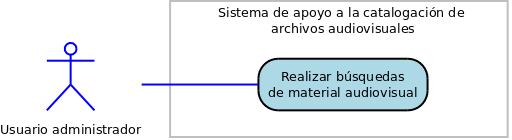
\includegraphics[width=0.8\textwidth]{CasoDeUso_Administrador_Busqueda.png}
\end{figure}

% Descripción
\textbf{Descipción: } Acción que permite realizar una búsqueda de material audiovisual.

% Precondiciones
\textbf{Precondiciones:} Estar en cualquiera de las páginas del sistema.

% Flujo Normal de Eventos (tabla)
\begin{adjustwidth}{-6em}{-6em}
	\begin{center}
		\begin{tabularx}{1.2\textwidth}{ | p{0.7cm} | X | p{0.7cm} | X | p{1.5cm} | }
			\hline
			\rowcolor{NewBlue} \multicolumn{5}{|c|}{\textbf{Flujo normal de eventos}} \\
			\hline
			\multicolumn{2}{|c|}{\textbf{Actor(es)}}	&	\multicolumn{2}{c|}{\textbf{Sistema}}	&	\textbf{Alterno} \\
			\hline
			\textbf{Paso}	&	\textbf{Acción}	&	\textbf{Paso}	&	\textbf{Acción}	&	\textbf{ID} \\
			\hline
			1 & 
			Escribir texto de búsqueda en el campo situado en la parte superior del navegador y presionar \textit{Enter} en el teclado o clic en el botón con el icono de lupa situado a la derecha &
			2 &
			El sistema realiza una búsqueda dentro de la base de datos con las coincidencias de las palabras escritas &
			E1 \\
			\hline
			& 
			&
			3 &
			El sistema muestra los resultados en pantalla utilizando la misma vista que los archivos audiovisuales por década (mostrando la portada, el título y el año) & 
			E2\\
			\hline
		\end{tabularx}
	\end{center}
\end{adjustwidth}

% Flujo de Excepcion de Eventos (tabla)
\begin{adjustwidth}{-6em}{-6em}
	\begin{center}
		\begin{tabularx}{1.2\textwidth}{ | p{0.6cm} | X | X | }
			\hline
			\rowcolor{NewBlue} \multicolumn{3}{|c|}{\textbf{Flujo excepcional de eventos}} \\
			\hline
			\textbf{ID}	&	\textbf{Descripción}	&	\textbf{Acción} \\
			\hline
			E1 &
			No hay conexión con la base de datos. &
			El sistema devuelve un mensaje de error de conexión. \\
			\hline
			E2 &
			No hay coincidencias de búsqueda en la base de datos. &
			El sistema muestra un texto indicando no hay resultados de la búsqueda. \\
			\hline
		\end{tabularx}
	\end{center}
\end{adjustwidth}

% Post-condiciones
\textbf{Postcondiciones:} El usuario es autodirigido a la página que muestra los audiovisuales resultantes de la búsqueda.

% Casos de prueba para flujo normal (tabla) y su prototipo (imagen)
%\begin{figure}[H]
%	\centering
%	\includegraphics[width=0.8\textwidth]{imagen.png}
%\end{figure}

\begin{adjustwidth}{-6em}{-6em}
	\begin{center}
		\begin{tabularx}{1.2\textwidth}{ | X | X | }
			\hline
			\rowcolor{NewBlue} \multicolumn{2}{|c|}{\textbf{Casos de prueba (Flujo normal)}} \\
			\hline
			\textbf{Entradas}	&	\textbf{Resultado esperado} \\
			\hline
			Escribir texto de búsqueda y presionar \textit{Enter} en el teclado o dar clic en el botón de búsqueda &
			El sistema muestra los audiovisuales resultantes en pantalla. \\
			\hline
		\end{tabularx}
	\end{center}
\end{adjustwidth}

% Casos de prueba para excepción de eventos (tabla) y su prototipo (imagen)
%\begin{figure}[H]
%	\centering
%	\includegraphics[width=0.8\textwidth]{imagen.png}
%\end{figure}

\begin{adjustwidth}{-6em}{-6em}
	\begin{center}
		\begin{tabularx}{1.2\textwidth}{ | p{0.6cm} | X | X | }
			\hline
			\rowcolor{NewBlue} \multicolumn{3}{|c|}{\textbf{Caso de prueba (Flujo excepcional)}} \\
			\hline
			\textbf{ID}	&	\textbf{Entrada}	&	\textbf{Resultado esperado} \\
			\hline
			E1 &
			No hay conexión con la base de datos. &
			El sistema devuelve un mensaje de error de conexión. \\
			\hline
			E2 &
			No hay coincidencias de búsqueda en la base de datos. &
			El sistema muestra un texto indicando no hay resultados de la búsqueda. \\
			\hline
		\end{tabularx}
	\end{center}
\end{adjustwidth}

\subsubsection{Agregar nuevo registro de material audiovisual}
% Actor
\textbf{Actor:} Usuario administrador

\subsubsection{Editar registro existente de material audiovisual}
% Actor
\textbf{Actor:} Usuario administrador

\subsubsection{Eliminar registro de material audiovisual}
% Actor
\textbf{Actor:} Usuario administrador

\subsubsection{Iniciar sesion como usuario del LAIS}
% Actor
\textbf{Actor:} Usuario administrador

\subsubsection{Cerrar sesion como usuario del LAIS}
% Actor
\textbf{Actor:} Usuario administrador

\subsubsection{Administración de usuarios del LAIS}
% Actor
\textbf{Actor:} Usuario administrador

% El formato anterior se repite como subseccion para cada caso de uso


\end{document}